\chapter{Experimental comparison}

We will perform an experimental comparison of selected ORM frameworks. In the form of unit tests, we will compare query capabilities across all 7 frameworks.

For each framework, we will create a set of unit tests performing pre-selected queries. Through these we will determine if the framework is capable of performing the query. 



We will only test read queries. They will provide us with enough information and metrics to compare the ORMs. Other non-read operations can be the subject of future work.

\section{Dataset}
% https://learn.microsoft.com/en-us/sql/samples/wide-world-importers-what-is?view=sql-server-ver16
To adequately test performance, we need a sufficiently large data set. Microsoft offers some pre-made open source datasets.
For this comparison, the Wide World Importers sample database \cite{microsoftWWI} has been selected.

The data set is fictional and does not correspond to a real company. The company description is as follows: ``Wide World Importers (WWI) is a wholesale novelty goods importer and distributor operating from the San Francisco bay area.``\cite{microsoftWWI}

The database contains four schemas: Application, Purchasing, Sales, Warehouse. For each query, we will select a suitable table and its columns that can best showcase the desired feature.

\section{Setup}
% database, docker, test project, .net
TODO Why we chose MSSQL

\section{Rules/assumptions} % TODO better name
As for query language, we will opt to use LINQ or any other available query language over raw SQL. 

For mapping database tables to entities, we will try using different methods to show the variety. 
As we have already seen, there are different approaches like attributes, fluent mapping by code or configuration files. 

If ORM supports caching entities, we will disable it so that our benchmarks are not affected. 
Another feature that could affect our results is change tracking. 
For example, EF Core tracks changes made to an entity, so that it can later perform an update. All our tests will only execute read operations, so change tracking would unnecessarily increase measured time or allocated memory.


\section{Selected queries}\label{sec:selected_queries}
Our goal is to test the query capabilities as broadly as possible. We want to create queries that use different conditions, result modifications, aggregations, relationships between tables, etc.

Each query type will contain an example of what the query should look like in raw SQL. The example can be used to directly query the test database to preview results. The example might be simplified for this text. Unit tests might use a different query language where available.

\subsection{A - Entity projection}
This group will test how well ORM can handle projecting table columns onto a user-defined entity or entities.

\subsubsection*{A1 Entity identical to a table} \label{query:a1}
The test will retrieve a table row and map it to an entity with properties identical to table columns. 
Table \texttt{Purchasing.PurchaseOrders} will be queried and one item retrieved based on its ID.

\begin{lstlisting}[language=SQL]
SELECT * FROM Purchasing.PurchaseOrders 
WHERE PurchaseOrderId = 25
\end{lstlisting}

\subsubsection*{A2 Limited entity}
The resulting entity will have less properties than table columns. Only the data we really need should be transferred. 
Table \texttt{Purchasing.Suppliers} will be queried and only columns related to supplier's contact info will be retrieved.

\begin{lstlisting}[language=SQL]
SELECT SupplierID, SupplierName, PhoneNumber, FaxNumber, WebsiteURL, ValidFrom, ValidTo 
FROM Purchasing.Suppliers 
WHERE SupplierID = 10
\end{lstlisting}

\subsubsection*{A3 Multiple entities from one table}
One table will be queried and the result will be divided into two different entities. 
Table \texttt{Purchasing.Suppliers} will be used again, from which we will retrieve contact information and bank account information into two separate entities. 

\begin{lstlisting}[language=SQL]
SELECT 
    SupplierId, SupplierName, PhoneNumber, FaxNumber, WebsiteURL, ValidFrom, ValidTo, 
    SupplierId, BankAccountName, BankAccountBranch, BankAccountCode, BankAccountNumber, BankInternationalCode 
FROM Purchasing.Suppliers 
WHERE SupplierID = 10
\end{lstlisting}

\subsubsection*{A4 Stored procedure result into entity}
This query will execute a stored procedure, limited by parameters, and load the result into an entity.
The executed stored procedure will be \texttt{Integration.GetOrderUpdates} with parameters LastCutoff and NewCutoff. 
We will limit the cut-off to a one-year range from 2014 to 2015. 66741 order updates should be returned.

This stored procedure returns columns with spaces in their names, for example, ``WWI Order ID``. As properties in the C\# language cannot contain spaces, it will be interesting to see how and if different frameworks can handle this.

\begin{lstlisting}[language=SQL]
EXEC WideWorldImporters.Integration.GetOrderUpdates 
@LastCutoff = '2014-01-01', @NewCutoff = '2015-01-01'
\end{lstlisting}

% \paragraph{} % TODO ASK - jak tady vrátit tenhle text zpět 
\subsubsection*{A Summary}
Queries \textbf{A1}, \textbf{A2}, and \textbf{A3} will fetch one row based on its ID. The measured time and memory allocation will then show the overhead of the ORM framework when mapping data to the resulting entities. Query \textbf{A4} returns a large number of results, so it is a first query that shows us the performance with high-volume data.

\subsection{B - Selection}
Probably the most common query operation is limiting results based on a condition. This set of queries will query table \texttt{Sales.OrderLines} with varied conditions.

\subsubsection*{B1 Selection over indexed column}
The query will retrieve one order line based on the ID of its order. The ID is foreign key with an index built over it.

\begin{lstlisting}[language=SQL]
SELECT * FROM Sales.OrderLines WHERE OrderID = 26866
\end{lstlisting}

\subsubsection*{B2 Selection over non-indexed column}
Unlike the first query, this one will fetch order lines filtered by a column without an index. The column that we will filter over will be unit price of the order line.
It is worth noting that it should not be relevant if a column is indexed or not for ORM comparison. Because all the queries will be performed over the same database system. We include both queries in case an interesting result appears.

\begin{lstlisting}[language=SQL]
SELECT * FROM Sales.OrderLines WHERE UnitPrice = 25
\end{lstlisting}

\subsubsection*{B3 Range query}
The previous queries filtered based on a single value, but a range of values is often desirable as well.
This query will select a subset of order lines with a column \texttt{PickingCompletedWhen} within a selected date range.

\begin{lstlisting}[language=SQL]
SELECT * FROM Sales.OrderLines 
WHERE PickingCompletedWhen 
BETWEEN '2014-12-20' AND '2014-12-31'
\end{lstlisting}

\subsubsection*{B4 In query}
When a range is not sufficient and we want specific values not fitting into an interval, we can provide a collection of values.
This query will return order lines belonging to orders with IDs 1, 10, 100, 1000, and 10000.

\begin{lstlisting}[language=SQL]
SELECT * FROM Sales.OrderLines 
WHERE OrderID IN (1, 10, 100, 1000, 10000)
\end{lstlisting}

\subsubsection*{B5 Text search}
This query will test a text search, looking for any order lines with description containing the word ``C++``.  The column does not have a full text search or any other index.

\begin{lstlisting}[language=SQL]
SELECT * FROM Sales.OrderLines 
WHERE Description LIKE '%C++%'
\end{lstlisting}

\subsubsection*{B6 Paging}
When filtering with a broad condition, a large amount of data might be returned. So we may opt to receive the data in batches. Another use case might be a paged table displayed to a user. For these a paging query with skip and take might be useful.
This query will fetch all order lines ordered by ID, but will skip first 1000 and take only next 50.

\begin{lstlisting}[language=SQL]
SELECT * FROM Sales.OrderLines 
ORDER BY OrderLineID 
OFFSET 1000 ROWS FETCH NEXT 50 ROWS ONLY
\end{lstlisting}

\subsection{C - Aggregation}
Aggregation functions are often used when performing calculations on data. We will test a select few.

\subsubsection*{C1 Count}
Count is very useful when we need to know the number of records that correspond to a specific condition. We will combine it with \texttt{GROUP BY} clause to retrieve distinct tax rates and the number of their occurrence.

\begin{lstlisting}[language=SQL]
SELECT TaxRate, COUNT(TaxRate) as Count 
FROM Sales.OrderLines 
GROUP BY TaxRate 
ORDER BY Count DESC
\end{lstlisting}

\subsubsection*{C2 Max}
Maximum and minimum are also commonly used. We will attempt to retrieve the maximum unit price for all order lines.

\begin{lstlisting}[language=SQL]
SELECT MAX(UnitPrice) FROM Sales.OrderLines
\end{lstlisting}

\subsubsection*{C3 Sum}
Aggregation functions also allow performing operations. In this test, we will combine the \texttt{SUM} function with a multiplication inside. The result will be the total price across all order lines.
\begin{lstlisting}[language=SQL]
SELECT SUM(Quantity * UnitPrice) FROM Sales.OrderLines
\end{lstlisting}

\subsection{D - Relations}
An important feature of ORM should be mapping relations. Our domain entities are often connected, representing relations in real life.
However, as we found out in our previous analysis, not all the selected frameworks support mapping relations. 

Our test data contain no one to one relation. There should be a small difference between mapping one to one and one to many. We will cover the other types in sufficient detail.

Some ORMs support lazy loading. That means loading entities in a relation only after accessing the corresponding collection. That would result in more queries being sent and a potential slowdown.
We will prevent this by setting the loading strategy to eager when possible.

\subsubsection*{D1 One to many}
In one to many relation we have one parent and multiple children. A parent entity should have a collection containing its children. Optionally, a child entity can have a reference to its parent.
In this test, we will use the relation between order and its order lines. We will fetch one specific order along with all its lines.

We need to verify all child entities were returned and the parent collection filled. 



\begin{lstlisting}[language=SQL]
SELECT o.*, ol.* FROM Sales.Orders o
LEFT JOIN Sales.OrderLines ol ON ol.OrderID = o.OrderID
WHERE o.OrderID = 530
\end{lstlisting}

\subsubsection*{D2 Many to many}
In many to many relation, both sides can be connected with multiple entities of the same type. Therefore, it will be represented by a collection on both sides. The collection can contain the entity directly, which makes it easier for developers to work with. If necessary, it can contain entities that represent the join table for this relationship.

This test will consist of two queries. We want to test accessing the relationship from both sides. The first query will fetch stock items with their stock groups. And the other one stock groups with their stock items.
The relationship is represented by a join table \texttt{Warehouse.StockItemStockGroups}. If possible, we will try to map this relation without a join entity in our tests.

\begin{lstlisting}[language=SQL]
SELECT si.*, sg.* FROM Warehouse.StockItems si
LEFT JOIN Warehouse.StockItemStockGroups sisg
    ON si.StockItemID = sisg.StockItemID
LEFT JOIN Warehouse.StockGroups sg
    ON sisg.StockGroupID = sg.StockGroupID
ORDER BY si.StockItemID
\end{lstlisting}
\begin{lstlisting}[language=SQL]
 SELECT sg.*, si.* FROM Warehouse.StockGroups sg
 LEFT JOIN Warehouse.StockItemStockGroups sisg
     ON sg.StockGroupID = sisg.StockGroupID
 LEFT JOIN Warehouse.StockItems si
     ON sisg.StockItemID = si.StockItemID
 ORDER BY sg.StockGroupID
\end{lstlisting}
The queries utilise left join, so we will get all stock items, even if they belong to no stock groups. And vice versa for the other query.

\subsubsection*{D3 One to many with optional relation}
In the D1 test case, the one to many relation was not optional. Each order has at least one order line. In the D2 test case, each item belonged to at least one category as well.
This test case will utilize an optional one to many relation between a customer and a transaction. 

\begin{lstlisting}[language=SQL]
SELECT c.*, ct.* FROM Sales.Customers c
LEFT JOIN Sales.CustomerTransactions ct
    ON c.CustomerID = ct.CustomerID
ORDER BY c.CustomerID
\end{lstlisting}

\subsection{E - Result modification}
This category will test modifying the result set. We will test sorting by a column and filtering distinct result values.

\subsubsection*{E1 Column sorting}
Although we have used sorting to order the results of some previous tests to get deterministic results, this test will focus solely on sorting.
We will sort all purchase orders by their expected delivery date and retrieve only the first one thousand.

\begin{lstlisting}[language=SQL]
SELECT TOP (1000) * FROM Purchasing.PurchaseOrders 
ORDER BY ExpectedDeliveryDate ASC
\end{lstlisting}

\subsubsection*{E2 Distinct results}
To test fetching only unique values, we will request all supplier references from purchase orders.

\begin{lstlisting}[language=SQL]
SELECT DISTINCT SupplierReference 
FROM Purchasing.PurchaseOrders
\end{lstlisting}

\subsection{F - Querying JSON}
Microsoft SQL Server supports storing and querying JSON data\cite{mssqljson}. It is worth testing if our selected ORMs support constructing queries into the stored JSON.
Table \texttt{Application.People} contains text columns storing JSON values.

During the static comparison, we found that none of the selected ORMs supports XML or any other data format. So we will not be testing for those.

\subsubsection*{F1 JSON object query}

Column \texttt{CustomFields} contains a JSON with many different values. In this test we will focus on property \texttt{Title}. We will query all people with a title set to ``Team Member``.
We will accomplish that using the \texttt{JSON\_VALUE} SQL function.

\begin{lstlisting}[language=SQL]
SELECT * FROM Application.People
WHERE JSON_VALUE(CustomFields, '$.Title') = 'Team Member'
ORDER BY PersonId
\end{lstlisting}

\subsubsection*{F2 JSON array query}

The first case covered querying a JSON object. This one will test querying inside a JSON array. Column \texttt{OtherLanguages} contains a JSON array containing language names.

\begin{lstlisting}[language=SQL]
SELECT * FROM Application.People
WHERE EXISTS (
    SELECT 1
    FROM OPENJSON(OtherLanguages)
    WHERE value = 'Slovak'
)
\end{lstlisting}

\subsection{G - Set operations}

In the last group we will test common set operations. Those are useful when having to combine two sets of data.

\subsubsection*{G1 Union}

Union will combine results from both queries. In this test, we will combine results from two different intervals of IDs and ensure that they are all present in the result.

\begin{lstlisting}[language=SQL]
SELECT SupplierID FROM Purchasing.Suppliers 
    WHERE SupplierID < 5
UNION
SELECT SupplierID FROM Purchasing.Suppliers 
    WHERE SupplierID BETWEEN 5 AND 10
ORDER BY SupplierID
\end{lstlisting}

\subsubsection*{G2 Intersection}

Intersection will include results that appear in both of the queries. We will try combining supplier IDs in two overlapping intervals and assert that only the overlap is included. 

\begin{lstlisting}[language=SQL]
SELECT SupplierID FROM Purchasing.Suppliers 
    WHERE SupplierID < 10
INTERSECT
SELECT SupplierID FROM Purchasing.Suppliers 
    WHERE SupplierID BETWEEN 5 AND 15
ORDER BY SupplierID
\end{lstlisting}

\subsection{H - Querying metadata}
In the last section, we will briefly test the ORM framework's ability to query information about the database itself. While not commonly used in applications, such data can be required in specific cases.
\subsubsection*{H1 Column data type}
The final query will attempt to retrieve the data type of a table column. All information about the database schema is available through \texttt{INFORMATION\_SCHEMA.COLUMNS} table. The selected column has \texttt{NVARCHAR} type. The table contains more information like nullability, maximum length, etc. But for demonstration purposes, this query should be sufficient.

\begin{lstlisting}[language=SQL]
SELECT DATA_TYPE FROM INFORMATION_SCHEMA.COLUMNS 
WHERE TABLE_SCHEMA = 'Purchasing'
    AND TABLE_NAME = 'Suppliers'
    AND COLUMN_NAME = 'SupplierReference'
\end{lstlisting}

\section{Summary of the selected queries}
We tried to pick as broad a selection of features as possible. 
We certainly did not cover all of them, but our set should be representative enough to give us a fair idea of how different ORMs perform. 

The tests perform queries across different tables and fetch different amounts of data. 
Measured time and memory allocation will not allow us to make any assumptions when comparing different test cases for the same ORM.
But we will be able to compare identical test cases across different ORMs.

We can expect to see a difference in time performance between micro frameworks made to be efficient and feature-rich macro frameworks.
The micro frameworks utilize raw SQL and have very little overhead. When using a macro framework, the LINQ query has to be compiled into SQL. Rich mapping capabilities may also cause significant slowdown. And extra features may even cause higher memory consumption.

\section{Implementation}
The comparison was implemented in the form of a Visual Studio solution, containing a project folder for each framework. Each project folder contains three projects - entities, feature tests, and performance benchmark. 


\usetikzlibrary{positioning, arrows}
\begin{center}
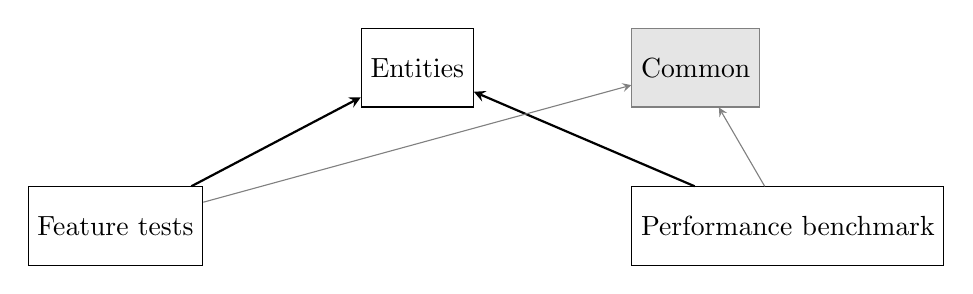
\begin{tikzpicture}[
    node distance=1cm and 2cm,
    every node/.style={draw, minimum width=1cm, minimum height=1cm, align=center},
    every path/.style={->, >=stealth},
    faded/.style={draw=gray, fill=gray!20},
    faded_arrow/.style={->, >=stealth, draw=gray}
]

  \node (E) {Entities};
  \node (C) [right=of E, faded] {Common};
  \node (FT) [below left=of E] {Feature tests};
  \node (PB) [below right=of E] {Performance benchmark};

  \draw[thick, ->, >=stealth] (FT) -- (E);
  \draw[thick, ->, >=stealth] (PB) -- (E);
  \draw[faded_arrow] (FT) -- (C);
  \draw[faded_arrow] (PB) -- (C);

\end{tikzpicture}
\end{center}

Common project is also included. It contains a single class handling loading the database connection string from a configuration file. There is no dependency between feature tests and performance tests. It could be argued that the code for queries could be extracted to a separate class to avoid duplication. But we have kept it duplicated to isolate unit tests from performance benchmarks. This structure is repeated for each of the seven frameworks we are examining. There is again no dependency between the different frameworks for isolation purposes.

\subsection{Entities}
Set of classes either mirroring a database table or containing a necessary subset of properties. The columns mapped always depend on the test they are being used in. The entities are POCOs (plain old CLR objects). The term is derived from POJO (plain old Java objects). \cite{Fowler2003POJO} It refers to classes that don't inherit from any base class or interface. And they are not tied to any specific framework.

Below is an example of a POCO class for a purchase order. Visibility modifiers and some properties were omitted for readability. 

% TODO Move explanation about what entities are to earlier section/introduction

\begin{lstlisting}[language=CSharp]
class PurchaseOrder
{
    int PurchaseOrderID { get; set; }
    int SupplierID { get; set; }
    DateTime OrderDate { get; set; }
    DateTime? ExpectedDeliveryDate { get; set; }
    string? Comments { get; set; }
}
\end{lstlisting}

Some frameworks like Dapper do not need any entity mapping and simply require the properties to match selected query columns. The purchase order entity could be used to load results of a query, but the query has to return columns with matching names, data types, and nullability.

More complex frameworks that do not just perform read queries need to know how to map an entity to a database table. The corresponding table might not even exist and is generated based on the entity. Such use case is central to domain-driven development\cite{FowlerDDD}.

Entity mapping might be done in multiple ways. The simplest form is no mapping. The framework would then guess table and column names, data types, nullability, etc. from the way an entity is named and declared. Clearly, that lacks details like numeric precision, constraints, and indices.
Those details could be specified by property and class attributes. That makes them tied to an entity, which could be a problem if we want to isolate the domain model from database access. 
Mapping through code or a configuration file allows separation and can be more expressive and powerful.

To showcase different approaches to mapping, we have tried to select a different method for each framework test. Mapping is usually compiled on application startup or first query and then cached. So performance should not be affected by a choice of mapping. Dapper does not use any mapping (as it does not support any). PetaPoco and RepoDB use attributes to declare table schema and name, and in some cases column names, the rest is inferred. For those two, mapping abilities are quite limited. LINQ to DB utilizes mapping by code through builder pattern. NHibernate has its proprietary mapping through files in XML format. Both versions of Entity Framework use attribute mapping combined with mapping through code. Their attribute mapping is much more powerful than those of PetaPoco and RepoDB, but in more complex cases, mapping by code has to be supplied.

First listing below shows attribute mapping in EF Core, where attributes are placed directly above classes and properties. In the second one, part of an XML mapping file for the same entity is shown. The verbosity of the mapping is noticeable.

\begin{lstlisting}[language=CSharp,basicstyle=\ttfamily\footnotesize]
[Table("PurchaseOrders", Schema = "Purchasing")]
class PurchaseOrder
{
    [Key]
    int PurchaseOrderID { get; set; }
}
\end{lstlisting}

\begin{lstlisting}[language=xml,basicstyle=\ttfamily\footnotesize]
<?xml version="1.0" encoding="utf-8" ?>
<hibernate-mapping xmlns="urn:nhibernate-mapping-2.2" namespace="NHibernateEntities">
    <class name="NHibernateEntities.PurchaseOrder, NHibernateEntities" table="PurchaseOrders" schema="Purchasing">
        <id name="PurchaseOrderID" column="PurchaseOrderID" type="int">
            <generator class="identity" />
        </id>
        <property name="SupplierID" not-null="true" />
        <property name="OrderDate" not-null="true" />
        ...
    </class>
</hibernate-mapping>
\end{lstlisting}

\subsection{Feature tests}

For each query defined in \autoref{sec:selected_queries}, a unit test in the form of an isolated method was implemented. Connection and other configuration are created outside of the test in a setup part. The method executes the query and correct results are asserted. Assertion checks the amount of results and their order. Each property is tested to contain correct data to ensure mapping was done correctly.

The example below shows Query A1 (\autoref{query:a1}) implemented for Dapper. A single purchase order is retrieved based on its ID, and its properties are checked for correct values. 
\begin{lstlisting}[language=CSharp]
[Fact]
public void A1_EntityIdenticalToTable()
{
    var order = connection.QuerySingle<PurchaseOrder>(
        "SELECT * FROM WideWorldImporters.Purchasing.PurchaseOrders WHERE PurchaseOrderId = @PurchaseOrderId",
        new { PurchaseOrderId = 25 }
    );

    Assert.Multiple(() =>
    {
        Assert.Equal(25, order.PurchaseOrderID);
        Assert.Equal(12, order.SupplierID);
        Assert.Equal(new DateTime(2013, 1, 5), order.OrderDate);
        ...
    });
}
\end{lstlisting}

\subsection{Performance benchmarks}
Feature tests can assert the correctness of returned results and overall functionality. But their execution time can greatly vary. There can be some overhead, coming from test initialization or assertions. The system the benchmarks are running on can also impact results.

To solve these problems we have used BenchmarkDotNet library\cite{BenchmarkDotNet}. It allows writing benchmark methods very similar to unit tests. In fact, they are completely identical to unit tests, the only differences are missing assertions and a different method attribute. It allows us to ``transform methods into benchmarks, track their performance, and share reproducible measurement experiments`` \cite{BenchmarkDotNet}. Work with the library was quite easy, it is very configurable and easy to run. 



It runs benchmark for each method multiple times. It starts with a few iterations which will not be included in the results. The first few ensure just-in-time compilation has taken effect, then multiple iterations without actually running the method code are started to compile overhead. The overhead is removed from the results, ensuring reliability. 


According to BenchmarkDotNet documentation\cite{BenchmarkDotNetHow} a single benchmark run consists of the following stages.
\begin{itemize}
    \item OverheadJitting - Measures benchmarking infrastructure compilation.
    \item WorkloadJitting - Measures benchmark method compilation.
    \item WorkloadPilot - Selects best iteration count based on heuristics.
    \item WorkloadWarmup - Runs several iterations before measuring to ensure factors like CPU caching or branch prediction are optimized.
    \item WorkloadActual - Actual measurements
    \item WorkloadResult - Result calculated from the actual run without the overhead.
\end{itemize}

TODO location of results

\section{Results}

\subsection{Features}

\subsection{Performance}
The final benchmark run was executed on a PC with the highest performance power plan while being constantly plugged in. Screen saving was turned off. The only applications running were those essential to the benchmark (database in Docker container and Visual Studio project). No other work was being done. Data further present are a result of that run and are available as an attachment.

The exact PC and runtime specifications are available below. This information is obtained from the benchmark run log. 
\begin{lstlisting}
BenchmarkDotNet v0.14.0, Windows 11 (10.0.22631.4890/23H2/2023Update/SunValley3)
AMD Ryzen 5 5600H with Radeon Graphics, 1 CPU, 12 logical and 6 physical cores
.NET SDK 9.0.101
  [Host]     : .NET 8.0.11 (8.0.1124.51707), X64 RyuJIT AVX2
  DefaultJob : .NET 8.0.11 (8.0.1124.51707), X64 RyuJIT AVX2
\end{lstlisting}

\begin{center}
    \captionof{table}{A1\_EntityIdenticalToTable}
    \sisetup{table-format=4.1, separate-uncertainty}
    \begin{tabular}{l S S S S S}
        \hline
        ORM & {Mean (\si{\micro\second})} & {Allocated (KB)} & {Gen0} & {Gen1} & {Gen2} \\
        \hline
        Dapper    & 750.2  & 6.24  & 0.0    & 0.0    & 0.0    \\
        PetaPoco  & 721.8  & 7.99  & 0.9766 & 0.0    & 0.0    \\
        RepoDB    & 747.5  & 8.77  & 0.9766 & 0.9766 & 0.0    \\
        Linq2db   & 839.2  & 12.74 & 0.9766 & 0.0    & 0.0    \\
        NHibernate & 742.1 & 36.06 & 3.9063 & 0.0    & 0.0    \\
        EF6       & 854.1  & 90.43 & 9.7656 & 0.0    & 0.0    \\
        EFCore    & 809.1  & 14.49 & 0.9766 & 0.0    & 0.0    \\
        \hline
    \end{tabular}
\end{center}


\clearpage
\begin{landscape}
\begin{table}
\centering
\caption{Performance benchmark results - Mean time (\unit{\micro\second})}
\label{tab:benchmark_results_time}
\begin{tabular}{lrrrrrrr}
\toprule
Namespace &    Dapper &  PetaPoco &    RepoDB &   Linq2db &  NHibernate &        EF6 &     EFCore \\
\midrule
A1\_EntityIdenticalToTable        &      750 &      722 &      748 &      839 &        742 &        854 &        809 \\
A2\_LimitedEntity                 &      718 &      726 &      735 &      858 &        958 &        882 &        799 \\
A3\_MultipleEntitiesFromOneResult &      736 &      736 &      745 &      898 &      1 001 &        945 &        832 \\
A4\_StoredProcedureToEntity       &  523 239 &  505 967 &  523 242 &  519 491 &    621 739 &    514 077 &    521 573 \\
B1\_SelectionOverIndexedColumn    &      744 &      759 &      762 &      868 &        817 &        905 &        806 \\
B2\_SelectionOverNonIndexedColumn &   43 612 &   41 100 &   43 052 &   43 708 &     86 419 &    125 169 &     48 016 \\
B3\_RangeQuery                    &   30 393 &   29 935 &   30 746 &   21 909 &     22 289 &     22 823 &     21 102 \\
B4\_InQuery                       &      856 &      855 &      876 &      954 &        945 &      1 408 &      1 147 \\
B5\_TextSearch                    &  747 728 &  747 721 &  745 551 &  745 319 &    746 464 &    746 264 &    744 754 \\
B6\_PagingQuery                   &    1 327 &    1 314 &    1 556 &    1 458 &      1 447 &      1 710 &      1 406 \\
C1\_AggregationCount              &   35 006 &   35 289 &  377 349 &   35 372 &     35 553 &     35 364 &     35 286 \\
C2\_AggregationMax                &    1 240 &    1 227 &    1 264 &    1 380 &      1 291 &      1 366 &      1 304 \\
C3\_AggregationSum                &   86 499 &   85 944 &   86 899 &   86 145 &     75 137 &     69 827 &     87 825 \\
D1\_OneToManyRelationship         &      781 &      770 &      806 &    2 997 &      1 042 &      1 581 &        895 \\
D2\_ManyToManyRelationship        &    4 584 &    4 480 &    6 031 &    9 383 &      5 940 &      6 913 &     14 964 \\
D3\_OptionalRelationship          &  187 693 &  172 030 &  393 631 &   91 326 &    533 489 &  1 993 146 &  2 548 411 \\
E1\_ColumnSorting                 &    4 725 &    4 622 &    4 963 &    4 845 &      6 316 &      6 204 &      4 885 \\
E2\_Distinct                      &    2 181 &    2 148 &    2 180 &    2 374 &      2 229 &      2 340 &      2 270 \\
F1\_JSONObjectQuery               &    1 459 &    1 478 &    1 457 &    1 552 &      1 494 &      1 490 &      1 544 \\
F2\_JSONArrayQuery                &    1 723 &    1 718 &    1 732 &    1 795 &      1 761 &      1 771 &      1 839 \\
G1\_Union                         &      728 &      715 &      723 &    1 580 &      1 538 &      1 613 &      1 561 \\
G2\_Intersection                  &      739 &      718 &      730 &    1 596 &      1 534 &      1 622 &      1 566 \\
H1\_Metadata                      &      851 &      843 &      844 &      925 &        866 &        899 &        814 \\
\bottomrule
\end{tabular}
\end{table}
\end{landscape}

\clearpage
\begin{landscape}
\begin{table}
\centering
\caption{Performance benchmark results - Allocated memory (KB)}
\label{tab:benchmark_results_memory}
\begin{tabular}{lrrrrrrr}
\toprule
Namespace &   Dapper & PetaPoco &   RepoDB &  Linq2db & NHibernate &        EF6 &     EFCore \\
\midrule
A1\_EntityIdenticalToTable        &      750 &      722 &      748 &      839 &        742 &        854 &        809 \\
A2\_LimitedEntity                 &      718 &      726 &      735 &      858 &        958 &        882 &        799 \\
A3\_MultipleEntitiesFromOneResult &      736 &      736 &      745 &      898 &      1 001 &        945 &        832 \\
A4\_StoredProcedureToEntity       &  523 239 &  505 967 &  523 242 &  519 491 &    621 739 &    514 077 &    521 573 \\
B1\_SelectionOverIndexedColumn    &      744 &      759 &      762 &      868 &        817 &        905 &        806 \\
B2\_SelectionOverNonIndexedColumn &   43 612 &   41 100 &   43 052 &   43 708 &     86 419 &    125 169 &     48 016 \\
B3\_RangeQuery                    &   30 393 &   29 935 &   30 746 &   21 909 &     22 289 &     22 823 &     21 102 \\
B4\_InQuery                       &      856 &      855 &      876 &      954 &        945 &      1 408 &      1 147 \\
B5\_TextSearch                    &  747 728 &  747 721 &  745 551 &  745 319 &    746 464 &    746 264 &    744 754 \\
B6\_PagingQuery                   &    1 327 &    1 314 &    1 556 &    1 458 &      1 447 &      1 710 &      1 406 \\
C1\_AggregationCount              &   35 006 &   35 289 &  377 349 &   35 372 &     35 553 &     35 364 &     35 286 \\
C2\_AggregationMax                &    1 240 &    1 227 &    1 264 &    1 380 &      1 291 &      1 366 &      1 304 \\
C3\_AggregationSum                &   86 499 &   85 944 &   86 899 &   86 145 &     75 137 &     69 827 &     87 825 \\
D1\_OneToManyRelationship         &      781 &      770 &      806 &    2 997 &      1 042 &      1 581 &        895 \\
D2\_ManyToManyRelationship        &    4 584 &    4 480 &    6 031 &    9 383 &      5 940 &      6 913 &     14 964 \\
D3\_OptionalRelationship          &  187 693 &  172 030 &  393 631 &   91 326 &    533 489 &  1 993 146 &  2 548 411 \\
E1\_ColumnSorting                 &    4 725 &    4 622 &    4 963 &    4 845 &      6 316 &      6 204 &      4 885 \\
E2\_Distinct                      &    2 181 &    2 148 &    2 180 &    2 374 &      2 229 &      2 340 &      2 270 \\
F1\_JSONObjectQuery               &    1 459 &    1 478 &    1 457 &    1 552 &      1 494 &      1 490 &      1 544 \\
F2\_JSONArrayQuery                &    1 723 &    1 718 &    1 732 &    1 795 &      1 761 &      1 771 &      1 839 \\
G1\_Union                         &      728 &      715 &      723 &    1 580 &      1 538 &      1 613 &      1 561 \\
G2\_Intersection                  &      739 &      718 &      730 &    1 596 &      1 534 &      1 622 &      1 566 \\
H1\_Metadata                      &      851 &      843 &      844 &      925 &        866 &        899 &        814 \\
\bottomrule
\end{tabular}
\end{table}
\end{landscape}